% Generated by GrindEQ Word-to-LaTeX 
\documentclass{article} % use \documentstyle for old LaTeX compilers

\usepackage[utf8]{inputenc} % 'cp1252'-Western, 'cp1251'-Cyrillic, etc.
\usepackage[croatian]{babel} % 'french', 'german', 'spanish', 'danish', etc.
\usepackage{amsmath}
\usepackage{amssymb}
\usepackage{txfonts}
\usepackage{mathdots}
\usepackage[classicReIm]{kpfonts}
\usepackage{graphicx}
\usepackage{enumitem}

% You can include more LaTeX packages here 

\title{Obrasci uporabe}
\pagenumbering{gobble}
\date{}


\begin{document}

%\selectlanguage{english} % remove comment delimiter ('%') and select language if required

\maketitle
\newpage

\section{Opis obrazaca uporabe}
\underline{UC1:Registracija}

\begin{itemize}
	\item \textbf{Glavni sudionik:} Korisnik
	
	
	\item \textbf{Cilj:} Stvoriti korisnički račun za pristup sustavu 
	
	
	\item \textbf{Sudionici}: Baza podataka
	
	
	\item \textbf{Preduvjet:} -
	
	
	\item \textbf{Opis osnovnog tijeka:} 
	\begin{enumerate}
		\item Korisnik odabire opciju za registraciju
		
		
		\item Korisnik unosi potrebne korisničke podatke
		
		
		\item Korisnik prima obavijest o uspješnoj registraciji
		
	\end{enumerate}
		\item \textbf{Opis mogućeg odstupanja:}

		\begin{enumerate}
		\item[$$2.a$$] Odabir već zauzetog korisničkog imena i/ili e-maila, unos korisničkog podatka u nedozvoljenom formatu ili pružanje neispravnoga e-maila
		
		\begin{enumerate}[label=\arabic*.]
		\item Sustav obavještava korisnika o neuspjelom upisu i vraća ga na stranicu za registraciju
		
		
		\item Korisnik mijenja potrebne podatke te završava unos ili odustaje od registracije
		\end{enumerate}
		\end{enumerate}
\end{itemize}
 

\noindent\underline{UC2:Prijava}

\begin{itemize}
	\item \textbf{Glavni sudionik:} Korisnik
	
	
	\item \textbf{Cilj:} Dobiti pristup korisničkom sučelju
	
	
	\item \textbf{Sudionici}: Baza podataka
	
	\item \textbf{Preduvjet:} Korisnik je registriran
	
	
	\item \textbf{Opis osnovnog tijeka:} 
	\begin{enumerate}
		\item Unos korisničkog imena i lozinke
		
		
		\item Potvrda o ispravnosti unesenih podataka
		
		
		\item Pristup korisničkim funkcijama
		
	\end{enumerate}
	\item \textbf{Opis mogućeg odstupanja:}
	
	\begin{enumerate}
		\item[$$1.a$$] Neispravno korisničko ime/lozinka
		
		\begin{enumerate}[label=\arabic*.]
			\item Sustav obavještava korisnika o neuspjelom upisu i vraća ga na stranicu za registraciju
			
		\end{enumerate}
	\end{enumerate}
\end{itemize}
 

\noindent\underline{UC3:Arhiviranje dokumenta}

\begin{itemize}
	\item \textbf{Glavni sudionik:} Računovođa
	
	
	\item \textbf{Cilj:} Arhivirati dokument u bazu podataka
	
	
	\item \textbf{Sudionici}: Baza podataka
	
	
	\item \textbf{Preduvjet:} Računovođa je prijavljen i revizor je provjerio dokument odgovarajućeg tipa
	
	
	\item \textbf{Opis osnovnog tijeka:} 
	\begin{enumerate}
		\item Računovođa dobiva popis dokumenata
		
		
		\item Računovođa bira dokument za arhiviranje
		
		
		\item Računovođa ima opciju poslati dokument direktoru na potpis
		
		\item Računovođa arhivira dokumente
		
		\item Dokumentu se dodjeljuje jedinstveni broj arhiva
		
	\end{enumerate}
\end{itemize}


\noindent\underline{UC3.1:Potpisivanje dokumenta}

\begin{itemize}
	\item \textbf{Glavni sudionik:} Direktor
	
	
	\item \textbf{Cilj:} Odobriti dokument kojeg je poslao računovođa
	
	
	\item \textbf{Sudionici}: Računovođa
	
	
	\item \textbf{Preduvjet:} Direktor je prijavljen i računovođa je poslao dokument kojeg treba potpisati
	
	
	\item \textbf{Opis osnovnog tijeka:} 
	\begin{enumerate}
		\item Direktor dobiva obavijest da treba potpisati dokument
		
		
		\item Direktor potpisuje dokument
		
		
		\item Računovođa dobiva obavijest da sada može arhivirati dokument
		
	\end{enumerate}
	\item \textbf{Opis mogućeg odstupanja:}
	
	\begin{enumerate}
		\item[$$2.a$$] Direktor nije potpisao dokument
		
		\begin{enumerate}[label=\arabic*.]
			\item Računovođa ne dobiva obavijest da može arhivirati dokument
			
		\end{enumerate}
	\end{enumerate}
\end{itemize}
  

\noindent\underline{UC4:Prikaz povijesti svih skeniranih dokumenata}

\begin{itemize}
	\item \textbf{Glavni sudionik:} Direktor
	
	
	\item \textbf{Cilj:}Prikazati povijest svih skeniranih dokumenata
	
	
	\item \textbf{Sudionici}: Baza podataka
	
	
	\item \textbf{Preduvjet:} -Direktor je prijavljen u sustav
	
	\qquad\qquad\quad  -Postoji barem jedan skenirani dokument
	
	\item \textbf{Opis osnovnog tijeka:} 
	\begin{enumerate}
		\item Direktor odabire opciju ,,Prikaz povijesti skeniranih dokumenata``
		
		
		\item Prikazuju se svi dokumenti koji su do tada skenirani
		
		
		
	\end{enumerate}
	\item \textbf{Opis mogućeg odstupanja:}
	
	\begin{enumerate}
		\item[$$1.a$$] Do tada nije skeniran ni jedan dokument
		
		\begin{enumerate}[label=\arabic*.]
			\item Sustav obavještava direktora da nema dokumenata za pokazati
			
		\end{enumerate}
	\end{enumerate}
\end{itemize}


\noindent\underline{UC5:Prikaz povijesti svojih skeniranih dokumenata}

\begin{itemize}
	\item \textbf{Glavni sudionik:} Zaposlenik
	
	
	\item \textbf{Cilj:}Prikazati povijest svojih skeniranih dokumenata
	
	
	\item \textbf{Sudionici}: Baza podataka
	
	
	\item \textbf{Preduvjet:} Korisnik je prijavljen u sustav i postoji barem jedan skenirani dokument od tog korisnika u bazi podataka
	
	
	\item \textbf{Opis osnovnog tijeka:} 
	\begin{enumerate}
		\item Korisnik odabire opciju ,,Prikaz povijesti skeniranih dokumenata``
		
		
		\item Prikazuju se svi dokumenti koje je prethodno skenirao
		
		
		
	\end{enumerate}
	\item \textbf{Opis mogućeg odstupanja:}
	
	\begin{enumerate}
		\item[$$1.a$$] Korisnik do tada nije skenirao ni jedan dokument
		
		\begin{enumerate}[label=\arabic*.]
			\item Sustav obavještava korisnika da nema dokumenata za pokazati
			
		\end{enumerate}
	\end{enumerate}
\end{itemize}
 

\noindent\underline{UC6:Provjera dokumenta}

\begin{itemize}
	\item \textbf{Glavni sudionik:} Revizor
	
	
	\item \textbf{Cilj:} Provjeriti dokument i proslijediti ga odgovarajućem računovođi
	
	
	\item \textbf{Sudionici}: Računovođa
	
	
	\item \textbf{Preduvjet:} Revizor je prijavljen i barem jedan zaposlenik je skenirao dokument i označio ga kao točan
	
	
	\item \textbf{Opis osnovnog tijeka:} 
	\begin{enumerate}
		\item Revizor dobiva popis dokumenata
		
		
		\item Revizor određuje kojem će računovođi poslati dokument
		
		
		\item Dokument se šalje odgovarajućem računovođi
		
	\end{enumerate}
	\item \textbf{Opis mogućeg odstupanja:}
	
	\begin{enumerate}
		\item[$$2.a$$] Revizor je skenirao taj dokument
		
		\begin{enumerate}[label=\arabic*.]
			\item Aplikacija automatski određuje kojem će računovođi poslati dokument
			
		\end{enumerate}
	\end{enumerate}
\end{itemize}


\noindent\underline{UC7:Skeniranje dokumenta}

\begin{itemize}
	\item \textbf{Glavni sudionik:} Korisnik
	
	
	\item \textbf{Cilj:} Skenirati dokument
	
	
	\item \textbf{Sudionici}: OCR
	
	
	\item \textbf{Preduvjet:} Korisnik je prijavljen
	
	
	\item \textbf{Opis osnovnog tijeka:} 
	\begin{enumerate}
		\item Korisnik odabire opciju "Skeniraj dokument"
		
		
		\item Otvara se aplikacija kamere mobitela
		
		
		\item Mobitel miruje minimalno 0,5 sekundi
		
		\item Aplikacija detektira i skenira dokument
		
		\item Korisniku se prikazuje sažetak dokumenta
		
	\end{enumerate}

\end{itemize}



\noindent\underline{UC7.1:Ocjena točnosti skeniranja}

\begin{itemize}
	\item \textbf{Glavni sudionik:} Korisnik
	
	
	\item \textbf{Cilj:} Procijeniti je li dokument točno skeniran i spremanje u bazu podataka
	
	
	\item \textbf{Sudionici}: Baza podataka
	
	
	\item \textbf{Preduvjet:} Korisnik je prijavljen i dokument je skeniran
	
	
	\item \textbf{Opis osnovnog tijeka:} 
	\begin{enumerate}
		\item Korisnik odabire je li dokument točno ili netočno skeniran
		
		
		\item Dokument i podatak o točnosti sprema se u bazu podataka
		
		
		\item Dokument se šalje odgovarajućem računovođi
		
	\end{enumerate}
	\item \textbf{Opis mogućeg odstupanja:}
	
	\begin{enumerate}
		\item[$$1.a$$] Zaposlenik je označio dokument kao točno skeniran
		
		\begin{enumerate}[label=\arabic*.]
			\item Dokument se šalje revizoru
			
			\item Dokument i podatak o točnosti sprema se u bazu podataka
			
		\end{enumerate}
	\end{enumerate}
\end{itemize}



\noindent\underline{UC8:Prikaz povijesti i statistike svih zaposlenika}

\begin{itemize}
	\item \textbf{Glavni sudionik:} Direktor
	
	
	\item \textbf{Cilj:} Prikazati povijest i statistiku zaposlenika
	
	
	\item \textbf{Sudionici}: Baza podataka
	
	
	\item \textbf{Preduvjet:} -Direktor je prijavljen u sustav
	
	\qquad\qquad\quad -Postoji barem jedan zaposlenik u bazi podataka
	
	
	\item \textbf{Opis osnovnog tijeka:} 
	\begin{enumerate}
		\item Direktor odabire opciju ,,Prikaz povijesti i statistike zaposlenika`` 
		
		
		\item Prikazuje se povijest i statistika zaposlenika
		
		
		
	\end{enumerate}
	\item \textbf{Opis mogućeg odstupanja:}
	
	\begin{enumerate}
		\item[$$1.a$$] U bazi podataka nema ni jednog zaposlenika
		
		\begin{enumerate}[label=\arabic*.]
			\item Sustav obavještava direktora da nema zaposlenika za pokazati
			
			
		\end{enumerate}
	\end{enumerate}
\end{itemize} 


\section{Dijagrami obrazaca uporabe}

\begin{figure}
	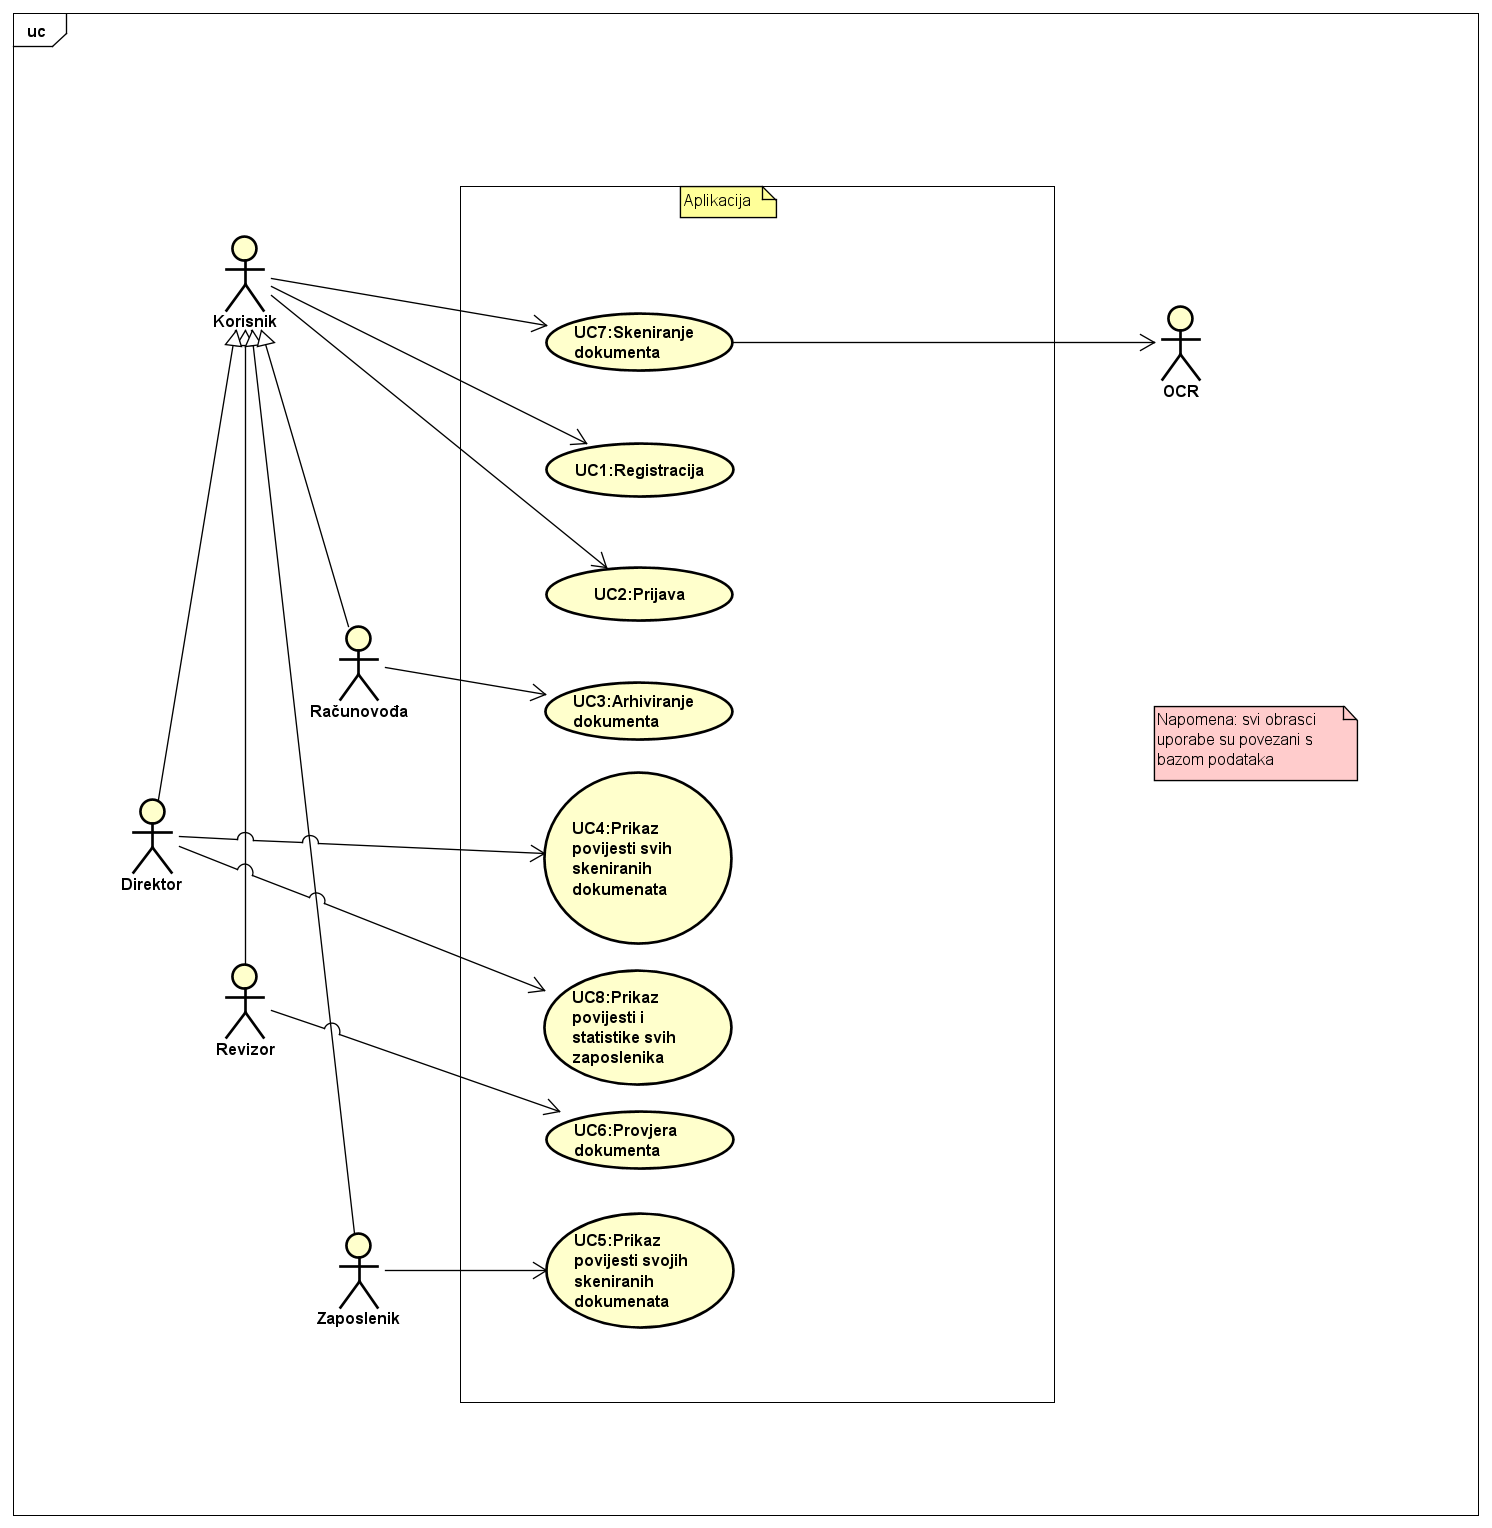
\includegraphics[width=\linewidth]{Aplikacija za digitalizaciju-cjelokupni pogled.png}
	\caption{Aplikacija za digitalizaciju-cjelokupni pogled}
\end{figure}

\begin{figure}
	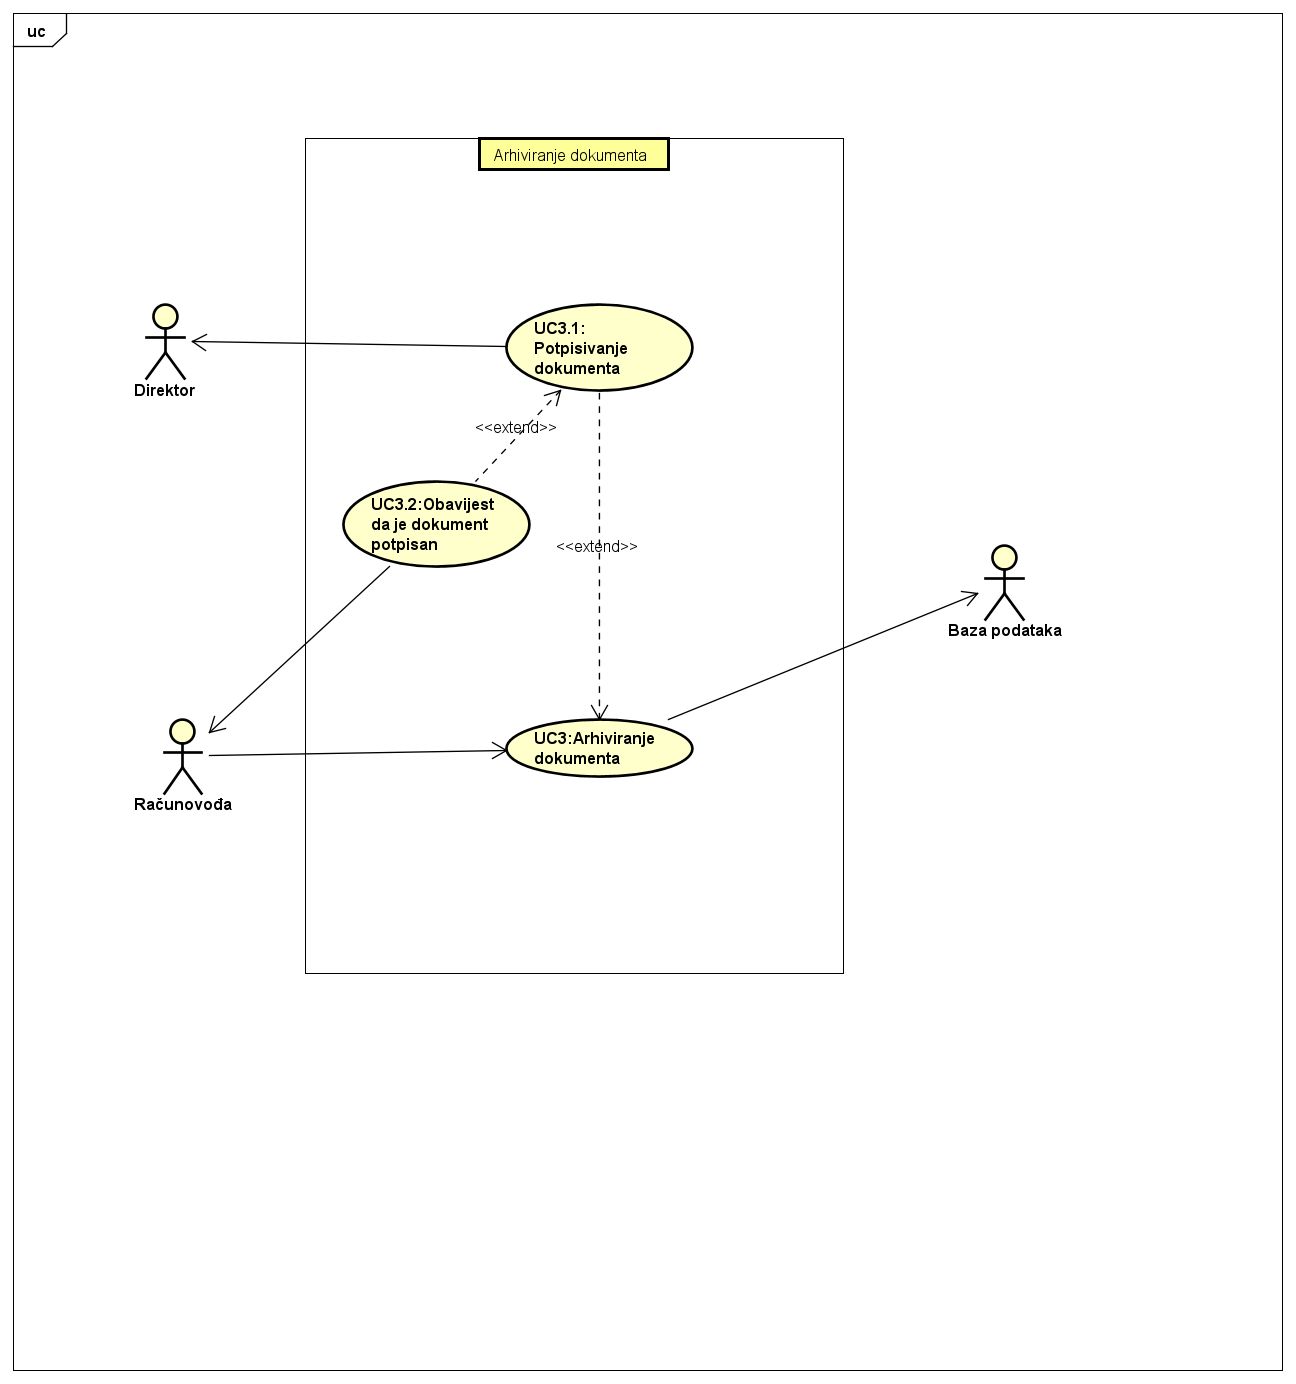
\includegraphics[width=\linewidth]{Aplikacija za digitalizaciju-arhiviranje dokumenta.png}
	\caption{Funkcionalnost-arhiviranje dokumenta}
\end{figure}

\begin{figure}
	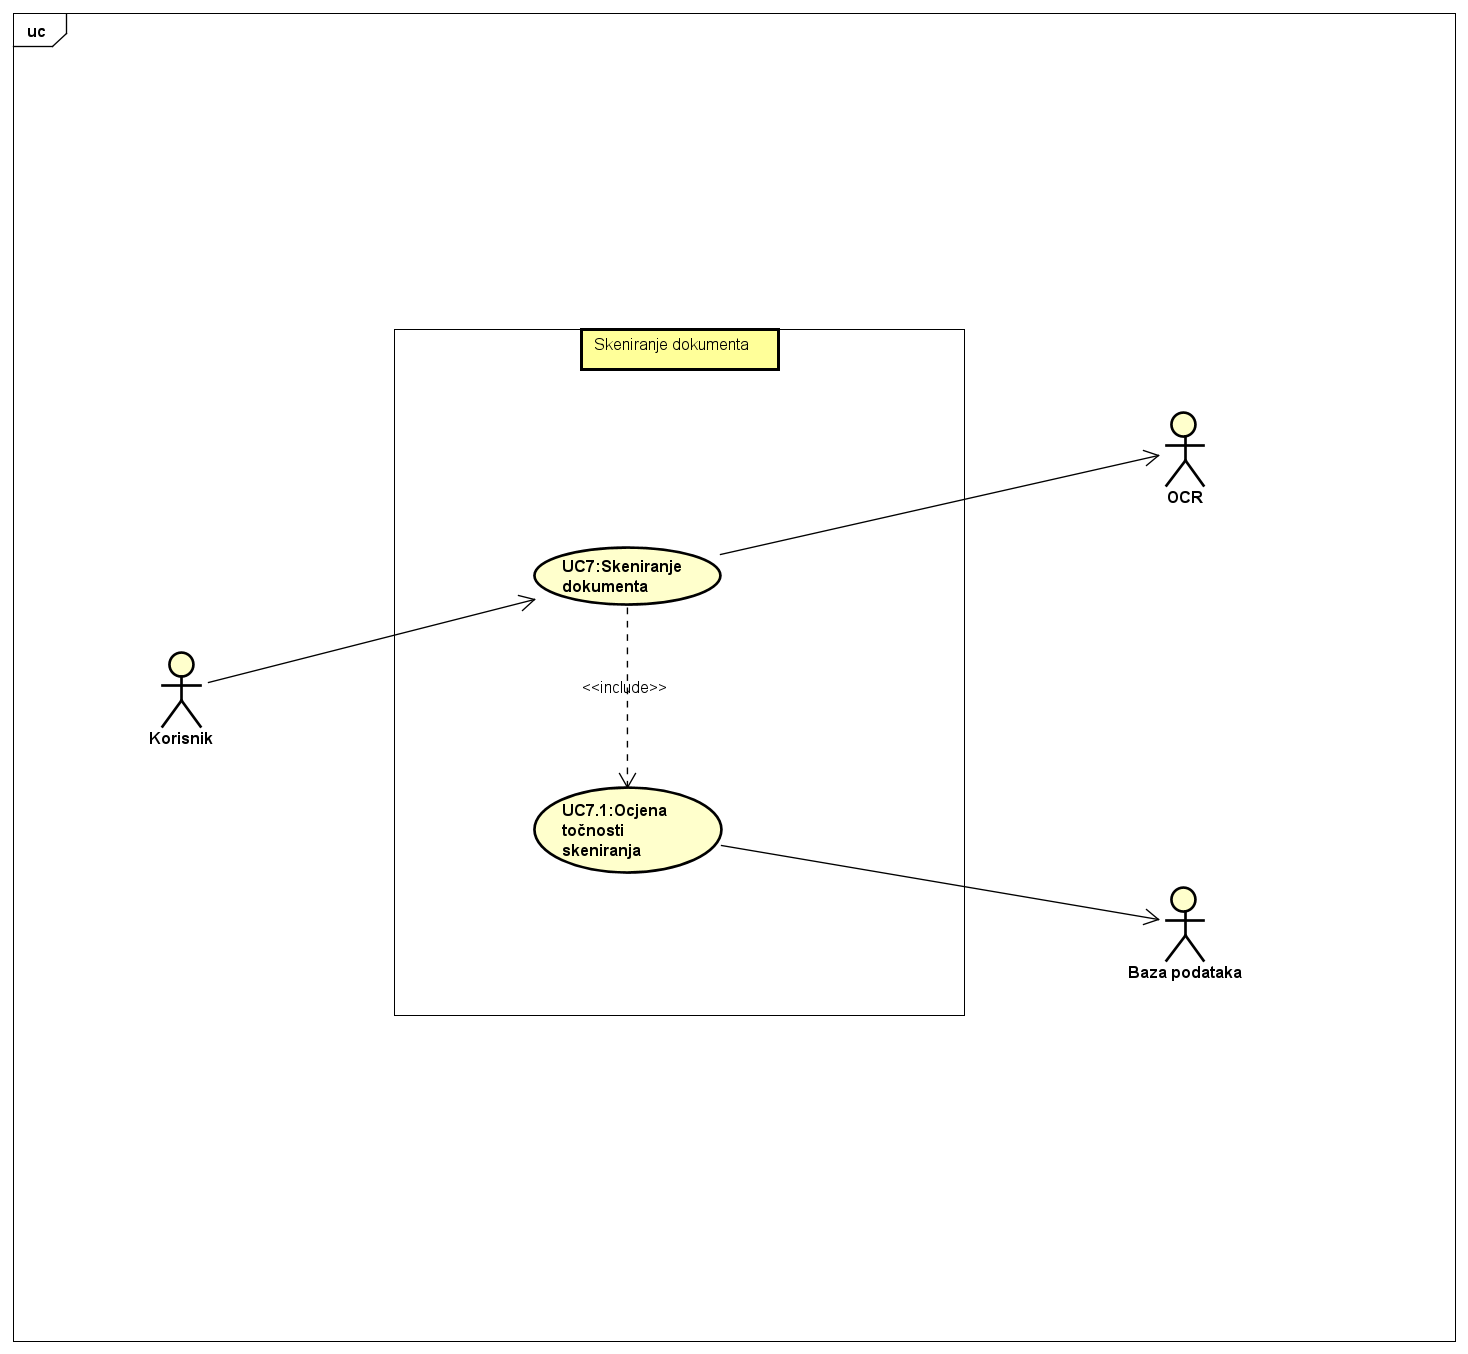
\includegraphics[width=\linewidth]{Aplikacija za digitalizaciju-skeniranje dokumenta.png}
	\caption{Funkcionalnost-skeniranje dokumenta}
\end{figure}

\end{document}

